%
% Complete documentation on the extended LaTeX markup used for Insight
% documentation is available in ``Documenting Insight'', which is part
% of the standard documentation for Insight.  It may be found online
% at:
%
%     http://www.itk.org/

\documentclass{InsightArticle}


%%%%%%%%%%%%%%%%%%%%%%%%%%%%%%%%%%%%%%%%%%%%%%%%%%%%%%%%%%%%%%%%%%
%
%  hyperref should be the last package to be loaded.
%
%%%%%%%%%%%%%%%%%%%%%%%%%%%%%%%%%%%%%%%%%%%%%%%%%%%%%%%%%%%%%%%%%%
\usepackage[dvips,
bookmarks,
bookmarksopen,
backref,
colorlinks,linkcolor={blue},citecolor={blue},urlcolor={blue},
]{hyperref}
% to be able to use options in graphics
\usepackage{graphicx}
% for pseudo code
\usepackage{listings}
% subfigures
\usepackage{subfigure}


%  This is a template for Papers to the Insight Journal. 
%  It is comparable to a technical report format.

% The title should be descriptive enough for people to be able to find
% the relevant document. 
\title{Improving features and performance of binary erode and dilate filters}

% Increment the release number whenever significant changes are made.
% The author and/or editor can define 'significant' however they like.
% \release{0.00}

% At minimum, give your name and an email address.  You can include a
% snail-mail address if you like.
\author{Ga\"etan Lehmann}
\authoraddress{Unit\'e de Biologie du D\'eveloppement et de la Reproduction, Institut National de la Recherche Agronomique, 78350 Jouy-en-Josas, France}

\begin{document}
\maketitle

\ifhtml
\chapter*{Front Matter\label{front}}
\fi


\begin{abstract}
\noindent
Binary erosion and dilation are the base filters of binary mathematical morphology.
In ITK 2.4.1 \verb$BinaryDilateImageFilter$ and \verb$BinaryErodeImageFilter$ implement
an efficient algorithm described in \cite{Nikopoulos2000}. However, those filter lack
support for boundary values, have a poor progress report, and can be quite inefficient
for complex 3D images.
\end{abstract}

% \tableofcontents

\section{Implementation}

Thread support have been completely removed: only a small part of the filter is treadable,
and sadly, it's the creation of the output image during the flooding stage which take the
most time to run, and it can't be threaded.

Adding boundary support was quite easy: the temporary image used internally is created
with an extra pixel on all borders, and the value of those pixel is set to foreground 
or background value, depending of the option set by the user.

To improve the progress report, the output pixels are set during the burning stage,
so there is no need to create a list with an unknown size.

To improve the performance, the output image is no more created with an output
iterator - the iterator is really inefficient in that case, because it copy all the neighbor pixels
in a buffer, while the filter need to access a small number of those pixels.

\section{Performance}

A timing test comparing performance on a $371 \times 371 \times 34$
image with a binary ball structuring element of size $20 \times 20 \times 7$ shows
that the new filters give better results than the old ones.

\begin{table}[htbp]
\centering
\begin{tabular}{cccccc}
\hline
border is foreground & foreground value & new erode & old erode & new dilate & old dilate \\
\hline
\hline
no & 100 & 18.4086 s & / & 11.7803 s & 59.7689 s \\
no & 200 & 13.5472 s & / & 2.65948 s & 8.28261 s\\
yes & 100 & 16.2584 s & 58.4875 s & 19.8128 s & /\\
yes & 200 & 11.7388 s & 17.3176 s & 10.7766 s & /\\
\hline
\end{tabular}
\caption{Execution times.\label{perf}}
\end{table}

\section{Examples}

Figures \ref{dilate}, \ref{erode} and \ref{dilateerode_1pt} show some examples of
of dilation and erosion with different structuring elements, and different parameters.

\begin{figure}[htbp]
\begin{center}
\subfigure[input image]{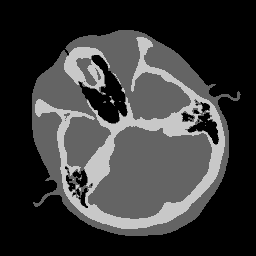
\includegraphics[scale=0.6]{2th_cthead1}}
\subfigure[foreground = 100, background = 0, border is background]{
\includegraphics[scale = 0.6]{dilate-100-0-0}}
\subfigure[foreground = 100, background = 0, border is foreground]{
\includegraphics[scale = 0.6]{dilate-100-0-1}}
\subfigure[foreground = 100, background = 150, border is background]{
\includegraphics[scale = 0.6]{dilate-100-150-0}}
\subfigure[foreground = 100, background = 150, border is foreground]{
\includegraphics[scale = 0.6]{dilate-100-150-1}}
\subfigure[foreground = 200, background = 0, border is background]{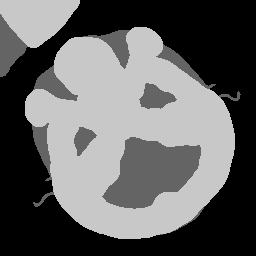
\includegraphics[scale = 0.6]{dilate-200-0-0}}
\subfigure[foreground = 200, background = 0, border is foreground]{
\includegraphics[scale = 0.6]{dilate-200-0-1}}
\subfigure[foreground = 200, background = 150, border is background]{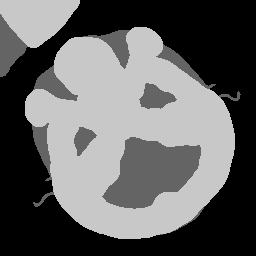
\includegraphics[scale = 0.6]{dilate-200-150-0}}
\subfigure[foreground = 200, background = 150, border is foreground]{
\includegraphics[scale = 0.6]{dilate-200-150-1}}
\caption{Dilation with a binary ball structuring element of radius 10.\label{dilate}}
\end{center}
\end{figure}

\begin{figure}[htbp]
\begin{center}
\subfigure[input image]{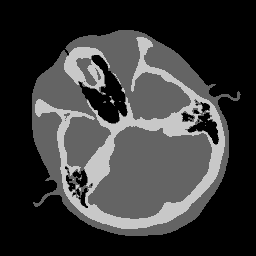
\includegraphics[scale=0.6]{2th_cthead1}}
\subfigure[foreground = 100, background = 0, border is background]{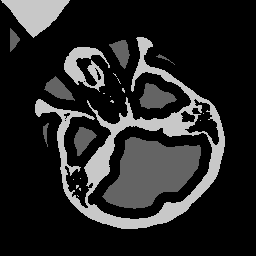
\includegraphics[scale = 0.6]{erode-100-0-0}}
\subfigure[foreground = 100, background = 0, border is foreground]{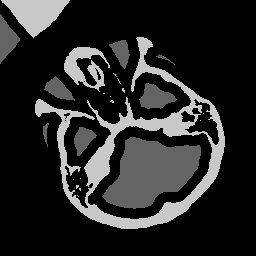
\includegraphics[scale = 0.6]{erode-100-0-1}}
\subfigure[foreground = 100, background = 150, border is background]{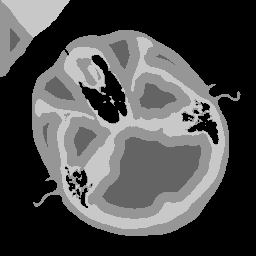
\includegraphics[scale = 0.6]{erode-100-150-0}}
\subfigure[foreground = 100, background = 150, border is foreground]{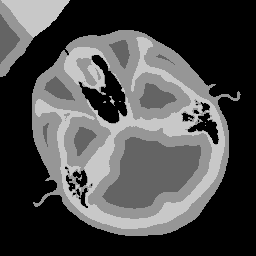
\includegraphics[scale = 0.6]{erode-100-150-1}}
\subfigure[foreground = 200, background = 0, border is background]{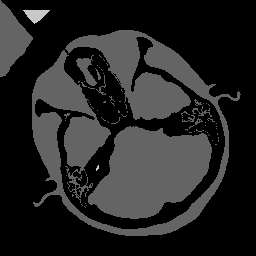
\includegraphics[scale = 0.6]{erode-200-0-0}}
\subfigure[foreground = 200, background = 0, border is foreground]{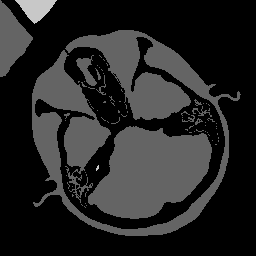
\includegraphics[scale = 0.6]{erode-200-0-1}}
\subfigure[foreground = 200, background = 150, border is background]{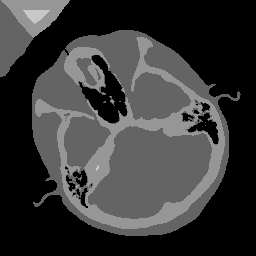
\includegraphics[scale = 0.6]{erode-200-150-0}}
\subfigure[foreground = 200, background = 150, border is foreground]{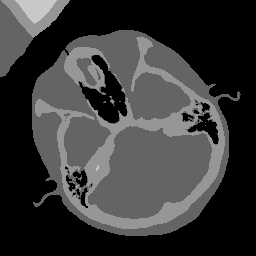
\includegraphics[scale = 0.6]{erode-200-150-1}}
\caption{Erosion with a binary ball structuring element of radius 10.\label{erode}}
\end{center}
\end{figure}

\begin{figure}[htbp]
\begin{center}
\subfigure[input image]{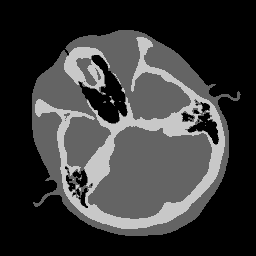
\includegraphics[scale=0.6]{2th_cthead1}}
\subfigure[foreground = 100, background = 0, border is background]{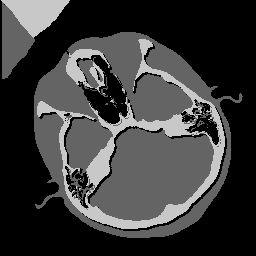
\includegraphics[scale = 0.6]{erode_1pt-100-0-0}}
\subfigure[foreground = 100, background = 0, border is foreground]{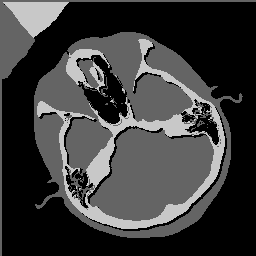
\includegraphics[scale = 0.6]{erode_1pt-100-0-1}}
\subfigure[foreground = 100, background = 150, border is background]{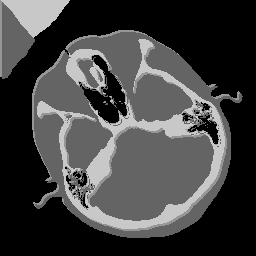
\includegraphics[scale = 0.6]{erode_1pt-100-150-0}}
\subfigure[foreground = 100, background = 150, border is foreground]{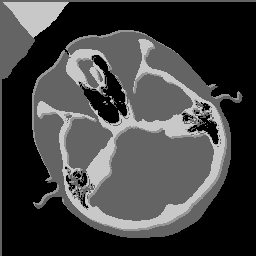
\includegraphics[scale = 0.6]{erode_1pt-100-150-1}}
\subfigure[foreground = 200, background = 0, border is background]{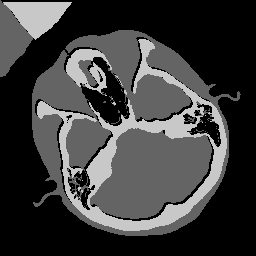
\includegraphics[scale = 0.6]{erode_1pt-200-0-0}}
\subfigure[foreground = 200, background = 0, border is foreground]{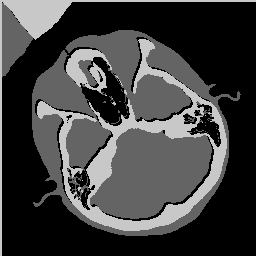
\includegraphics[scale = 0.6]{erode_1pt-200-0-1}}
\subfigure[foreground = 200, background = 150, border is background]{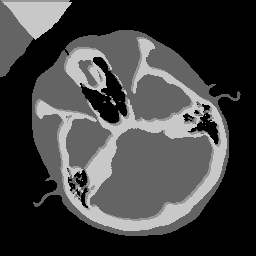
\includegraphics[scale = 0.6]{erode_1pt-200-150-0}}
\subfigure[foreground = 200, background = 150, border is foreground]{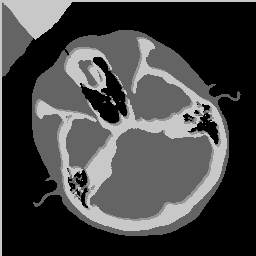
\includegraphics[scale = 0.6]{erode_1pt-200-150-1}}
\caption{Dilation and erosion with a structuring element with only one point.\label{dilateerode_1pt}}
\end{center}
\end{figure}


\section{Code sample}

\small \begin{verbatim}
#include "itkImageFileReader.h"
#include "itkImageFileWriter.h"
#include "itkCommand.h"
#include "itkSimpleFilterWatcher.h"

#include "itkBinaryDilateImageFilter.h"
#include "itkBinaryBallStructuringElement.h"
#include "itkNeighborhood.h"


int main(int, char * argv[])
{
  const int dim = 2;
  
  typedef unsigned char PType;
  typedef itk::Image< PType, dim > IType;

  typedef itk::ImageFileReader< IType > ReaderType;
  ReaderType::Pointer reader = ReaderType::New();
  reader->SetFileName( argv[4] );

  typedef itk::BinaryBallStructuringElement< PType, dim > SRType;
  SRType kernel;
  kernel.SetRadius( 10 );
  kernel.CreateStructuringElement();

  typedef itk::BinaryDilateImageFilter< IType, IType, SRType > FilterType;
  FilterType::Pointer filter = FilterType::New();
  filter->SetInput( reader->GetOutput() );
  filter->SetKernel( kernel );
  filter->SetForegroundValue( atoi(argv[1]) );
  filter->SetBackgroundValue( atoi(argv[2]) );
  filter->SetBoundaryIsForeground( atoi(argv[3]) );

  itk::SimpleFilterWatcher watcher(filter, "filter");

  typedef itk::ImageFileWriter< IType > WriterType;
  WriterType::Pointer writer = WriterType::New();
  writer->SetInput( filter->GetOutput() );
  writer->SetFileName( argv[5] );

  writer->Update();

  return 0;
}
\end{verbatim} \normalsize

\section{Conclusion}
The new proposed filters outperform the old ones, and provide more features.
However, it is surely possible to improve the performance of the new filters.
The creation of the output image still use lots of time. An iterator which
put only the neighbors in a buffer may be a great help in that case.


\section{Acknowledgments}
I thank Dr Pierre Adenot and MIMA2 confocal facilities
(\url{http://mima2.jouy.inra.fr}) for providing image samples.

I also thank Jerome SCHMID for his explanations, and for his first work
on those filters.


\appendix



\bibliographystyle{plain}
\bibliography{InsightJournal,Article}
\nocite{ITKSoftwareGuide}

\end{document}

